\section{Relation to Classical Stability, Consistency, and Conformal Prediction}
\label{sec:consistency}

It is worth pausing to say what these finite worst-case separations do
\emph{not} imply. Classical nearest-neighbor theory studies risk under a
distributional sampling model and asks whether the learned classifier converges
to the Bayes rule or to a near-optimal risk level as sample size grows
\cite{cover1967nearest,cover1968estimation,stone1977consistent,devroye1996probabilistic}. Our results
operate on a different axis: fixed finite samples, deterministic tie-breaking,
and worst-case one-perturbation sensitivity.

The present indicators are suprema over fixed samples, perturbations, and
query-label pairs; consistency results instead concern risk under a sampling
distribution and asymptotic regimes for $n$ and often $k=k_n$.

\begin{figure}[t]
    \centering
    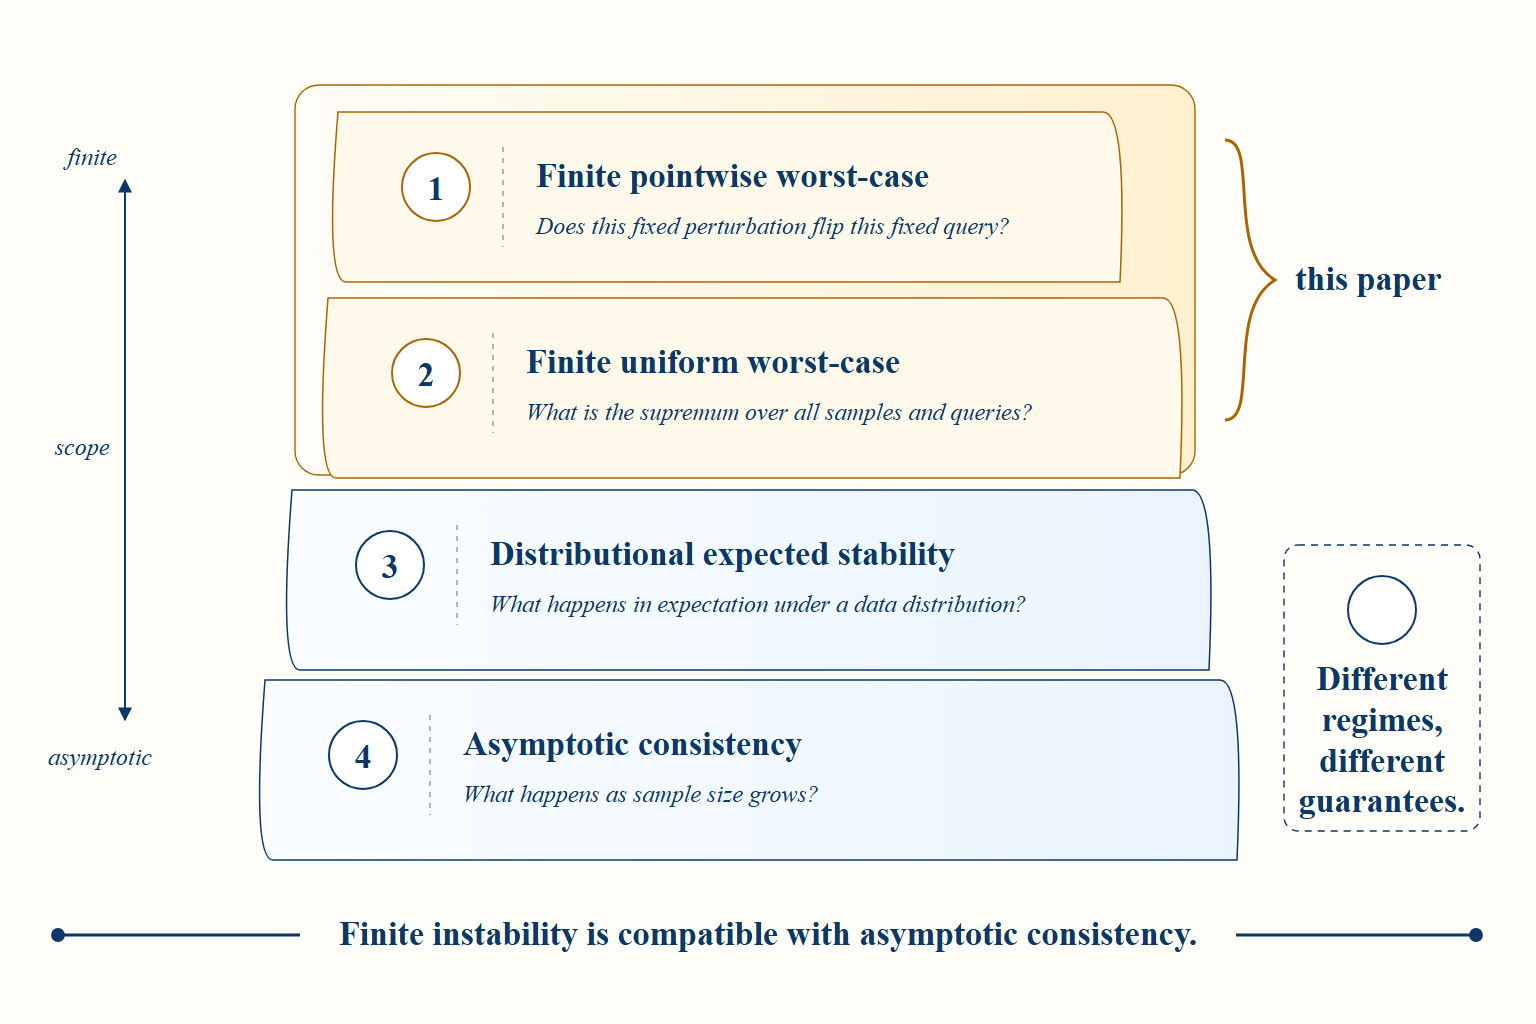
\includegraphics[width=0.84\linewidth]{outputs/figures/recreated_fig10.png}
    \caption{Finite worst-case perturbation sensitivity, classical asymptotic
    consistency, and conformal-style conditional validity live in different
    analytical regimes. The present paper sits in the first regime.}
    \label{fig:regimes-map}
\end{figure}

There is therefore no contradiction between the statements
``deterministic finite $1$-NN can be replace-one unstable at a fixed query''
and ``$k$-NN is consistent under the usual asymptotic hypotheses.'' The former
is a local combinatorial fact about a chosen finite configuration. The latter is
a distributional limit theorem. Both can be true simultaneously, and in the present paper they are.

This distinction also helps orient the relation to conformal prediction and
LOO-style calibration analyses. In those literatures, one often studies how
deleting or exchanging points affects a prediction set, a conformity score, or a
coverage certificate under exchangeability or training-conditional assumptions.
Those are important questions, but they are not identical to the present
0--1-loss perturbation calculus for deterministic $k$-NN. Our witness results
should therefore be read as a mechanism-level complement to that literature,
not as a replacement for it.

This has a concrete implication: if one wants a stability notion for a local
learner, one should first decide whether the goal is generalization control,
cross-validation behavior, adversarial local robustness, or training-conditional
prediction stability. The same phrase ``change one sample point'' does not serve
all four purposes equally well.
